%Based on RTU EEF guidelines for bachelor thesis
%https://www.rtu.lv/writable/public_files/RTU_025.pdf

\documentclass[12pt,fleqn,titlepage,oneside]{article}

%Page margins according to guidelines
\usepackage[a4paper,top=30mm,right=15mm,bottom=30mm,left=35mm]{geometry}
%Indent first paragraph after section header
\usepackage{indentfirst}
%Set space between lines (1, 1.5, 2)
\usepackage{setspace}
%Set paragraph first line indent according to guidelines
\setlength{\parindent}{15mm}

%Select alternative section titles
\usepackage{titlesec}
%Double line spacing after section title
\titlespacing*{\section}
	{0pt}{\baselineskip}{2\baselineskip}
%Normal spacing around subsection title
\titlespacing*{\subsection}
	{0pt}{\baselineskip}{\baselineskip}

%Change enumerate number formatting
\usepackage{enumitem}
%More enumeration options
\usepackage{moreenum}

%Set table of contents depth to subsections
\setcounter{tocdepth}{2}
%Control table of contents, figures, etc
\usepackage{tocloft}
%Add " lpp." after section page number in table of contents
\renewcommand{\cftsecafterpnum}{\textbf{ lpp.}}
%Add " lpp." after subsection page number in table of contents
\renewcommand{\cftsubsecafterpnum}{ lpp.}

%Improved interface for floating objects
\usepackage{float}
%Support for sub-captions
\usepackage{subcaption}
%Produces figures which text can flow around
\usepackage{wrapfig}
%Control float placement with \FloatBarrier
\usepackage{placeins}

%AMS mathematical facilities for LaTeX
\usepackage{amsmath}
%Mathematical tools to use with amsmath
\usepackage{mathtools}
%Typeset physical units following the rules of the International System of Units (SI)
\usepackage{SIunits}
%Code formatting
\usepackage{listings}

%Tabulars with adjustable-width columns
\usepackage{tabularx}
%Driver-independent color extensions for LaTeX and pdfLaTeX
\usepackage{xcolor}
%Enhanced support for graphics (\includegraphics)
\usepackage{graphicx}

%Create PostScript and PDF graphics in TeX
\usepackage{tikz}
\usetikzlibrary{positioning,fit}
%Draw electrical networks with TikZ
\usepackage[EFvoltages]{circuitikz}
%Easy generation of timing diagrams as TikZ pictures
\usepackage{tikz-timing}
%Create normal/logarithmic plots in two and three dimensions
\usepackage{pgfplots}
\pgfplotsset{compat=newest}

%Accept different input encodings
\usepackage[utf8]{inputenc}

%Add section number to equations, figures and tables
\numberwithin{equation}{section}
\numberwithin{figure}{section}
\numberwithin{table}{section}

%Set caption label names according to guidelines
\renewcommand{\contentsname}{Saturs}
\renewcommand{\figurename}{att.}
\renewcommand{\tablename}{tabula}
%Set caption label format according to guidelines
\DeclareCaptionLabelFormat{tableLabelFormat}{#2 #1}
\DeclareCaptionLabelFormat{figureLabelFormat}{#2 #1}
\DeclareCaptionLabelSeparator{figureLabelSeperator}{ }
\DeclareCaptionFormat{mine}{\raggedleft #1\\\centering #3}%
\captionsetup[table]{labelformat=tableLabelFormat, singlelinecheck=off, format=mine}
\captionsetup[figure]{labelsep=figureLabelSeperator, labelformat=figureLabelFormat}

%Used for drawing a dashed vertical line from a point to the x axis in pgfplots
\newcommand{\vertLineFromPoint}[1]{
  \draw[dashed] 
  (#1) -- (#1|-{rel axis cs:0,0})
}
%Used for drawing a dashed horizontal line  from a point to the y axis in pgfplots
\newcommand{\horLineFromPoint}[1]{
  \draw[dashed] 
  (#1) -- (#1-|{rel axis cs:0,0})
}

\tikzstyle{block} = [draw, fill=white, rectangle, minimum height=3em, minimum width=6em]

%Variables used in the document
\newcommand{\authorName}{Valters Melnalksnis}
\newcommand{\authorId}{161REC035}

%Bibliography
\usepackage[language=latvian]{biblatex}
\BiblatexLatvianWarningOff
\addbibresource{bibliography.bib}

%PDF hyperlinks, navigation, etc.
\usepackage{url}
\usepackage{hyperref}
\hypersetup{
	breaklinks=true,
	bookmarks=true,
	unicode=true,
	hidelinks
}

%Split document in multiple files
\usepackage{subfiles}

%Render to external, files to minimize compile time
\usetikzlibrary{external}
\tikzset{external/optimize=false}
\usepgfplotslibrary{external}
\tikzexternalize

\begin{document}
\begin{titlepage}
	\centering
	\doublespacing
	{\Large \textbf{Rīgas Tehniskā Universitāte}}
	
	{Elektrotehnikas un vides inženierzinātņu fakultāte\\}
	{Industriālās elektronikas un elektrotehnikas institūts\\}
	{Industriālās elektronikas un elektrotehnoloģiju katedra\par}
	\vspace{2cm}
	
	\onehalfspacing
	{\Large \textbf{\authorName}\\}
	Profesionālā bakalaura adaptronikas studiju programmas students,\\
	stud. apl. nr. \authorId
	\vspace{2cm}
	
	{\huge 18650 tipa bateriju elementu ietilpības pētīšanas iekārtas izpēte un izstrāde\par}
	
	\doublespacing
	{\Large Bakalaura darbs ar projekta daļu\par}
	\onehalfspacing
	\vspace{6cm}
	
	\raggedleft
	Zinātniskais vadītājs\\
	RTU IEEI pētnieks\\
	Kristaps Vītols
	
	\centering
	\vfill
	Rīga, \the\year
\end{titlepage}

\onehalfspacing
\FloatBarrier
\newpage
\setcounter{page}{2}
\section*{\MakeUppercase{Anotācija}}

\newpage

\section*{\MakeUppercase{Abstract}}

\newpage

\doublespacing
\tableofcontents
\onehalfspacing
\newpage

\addcontentsline{toc}{section}{\texorpdfstring{\MakeUppercase{Ievads}}{Ievads}}
\section*{\texorpdfstring{\MakeUppercase{Ievads}}{Ievads}}

\FloatBarrier
\newpage

%TODO Nosaukums ???
\section{\texorpdfstring{\MakeUppercase{Teorijas izpēte}}{Teorijas izpēte}}

\subsection{Baterijas}

Baterija ir viena vai vairākas virknē slēgtas elektroķīmiskās šūnas.
Baterijas galvenokārt var iedalīt divās grupās - primārajās un sekundārajās.
Primārās jeb vienreizējās lietošanas baterijas var tikt izmantotas (izlādētas) tikai vienu reizi, jo izlādes gaitā elektrods tiek neatrgiežami bojāts.
Savukārt sekundārās jeb uzlādējamās baterijas pēc izlādes ir iespējams vairākkārt uzlādēt pievienojot ārēju barošanas avotu.
Primārajām baterijās parasti ir lielāka specifiskā enerģija, savukārt sekundārajām ir lielāka maksimālā izlādes strāva.

Galvenie bateriju parametri:
\begin{itemize}
	\item Elektrolīta veids
	\item Elektrodu veids
	\item Nominālais, maksimālais un minimālais spriegums
	\item Maksimālā uzlādes/izlādes strāva
	\item Pašizlādes ātrums
	\item Iekšējā presetība
	\item Ietilpība ampērstundās $(Ah)$
	\item C-reitings jeb maksimālā strāva kā koeficients no ampēriem no ietilpības ampērstundās
\end{itemize}

\subsection{18650 šūnas}

18650 (vai arī 168A) šūnu tipiskā ietilpība ir no 1500 līdz 3500 $mAH$, nominālais spriegums 3.7 $V$,
diametrs 18 $mm$ un garums 65 $mm$.\cite{18650cell}
Lai gan fiziskie izmēri ir standartizēti, šūnām ar izvirzītu pozitīvo termināli var atšķirties izvirzījuma izmēri,
līdz ar to tās var būt nesaderīgas ar ierīcēm.

\subsubsection{Uzlāde}

Vienas šūnas uzlādei ir divi posmi - konstantas strāvas un konstanta sprieguma.
Šie posmi veidojas no diviem šūnas parametriem - maksimālās uzlādes strāvas un maksimālā sprieguma.

Uzlādējot vairākas virknē slēgtas šūnas vēl nepieciešams balansēt uzlādi starp šūnām, 
jo tās var uzlādēties dažādos ātrumos atšķirīgu iekšējo pretestību dēļ.

\subsubsection{Izlāde}

\subsection{Līdzīgas iekārtas}

\subsubsection{Eagle Eye}

\subsubsection{PEC ACT0505}

ACT0505 

\subsubsection{SkyRC}

Spēj izlādēt 2-8 virknē slēgtas LiPo/LiFe/LiHv šūnas, 6-23 NiMH/NiCD šūnas vai 6-32V Pb baterijas.
Ir konstantas strāvas un jaudas režīmi, USB savienojums ar Windows programmatūru.

\begingroup
\renewcommand{\arraystretch}{1.25}
\begin{table}[h]
	\caption{SkyRc bateriju izlādes sitēmu parametri} 	
	\label{tab:skyrcdischarge}
	\centering
	\begin{tabularx}{\linewidth}{ 
		>{\setlength\hsize{1\hsize}\centering}X| 
		>{\setlength\hsize{0.3\hsize}\centering}X| 
		>{\setlength\hsize{0.3\hsize}\centering}X| 
		>{\setlength\hsize{0.3\hsize}\centering}X}
		Parametrs								& Mērvienība	& BD200\cite{bd200}		& BD250\cite{bd250}	\tabularnewline
		\hline
		Min. Spriegums                        	& $V$     		& $5.40$				& $5.40$ 			\tabularnewline
		Max. Spriegums                        	& $V$     		& $35.00$				& $35.00$			\tabularnewline
		Max. Jauda                            	& $W$     		& $200$					& $250$				\tabularnewline
		Max. Strāva                           	& $A$     		& $30$					& $35$				\tabularnewline
		Precizitāte, strāva $< 10A$           	& $\pm mA$		& $60$					& $60$				\tabularnewline
		Precizitāte, strāva $> 10A$           	& $\pm\%$ 		& $2$					& $3$				\tabularnewline
		Precizitāte, spriegums $< 10V$        	& $\pm mV$		& $60$					& $80$				\tabularnewline
		Precizitāte, $10V <$ spriegums $< 20V$	& $\pm mV$		& $120$					& $120$				\tabularnewline
		Precizitāte, spriegums $> 20V$        	& $\pm mV$		& $160$					& $160$	
	\end{tabularx}
\end{table}
\endgroup

\subsubsection{Amperis}

\subsubsection{RCDischarger}

\subsubsection{SBSBattery}

\clearpage
\section{\texorpdfstring{\MakeUppercase{Izstrādājamās sistēmas analīze}}{Izstrādājamās sistēmas analīze}}

Šunu testēšanas sistēma sastāvēs no viena vadības moduļa un vairākiem testēšanas moduļiem.
Vadības moduļa galvenās funckijas būs testa datu uzkrāšana un katras šūnas testa procesa vadība.
Savukārt testēšanas modulis sastāves no mērīšanas, uzlādes un izlādes moduļiem. Mērīšanas moduļi mērīs baterijas parametrus (spriegumu, strāvu un temperatūru), kā arī pieslēgs vai atvienos uzlādes un izlādes moduļus no baterijas.
Vadības modulis komunicēs ar mērīšanas moduļiem, kuri savukārt komunicēs ar attiecīgajiem uzlādes un izlādes moduļiem. 

% Vai šim paragrāfam jābūt pie teorijas vai prakses?
Testēšanas moduļi tiks slēgti paralēli, līdz ar to to skaitu ierobežos tikai izvēlētais komunikācijas protokols un tā ātrums.
Divi iespējamie komunikācijas protokoli ir I\textsuperscript{2}C (Inter-Integrated Circuit) un SPI (Serial Peripheral Interface) daisy-chain konfigurācijā.
I\textsuperscript{2}C komunikācija notiek starp vienu master un vienu slave ierīci master ierīcei norādot slave ierīces adresi.
I\textsuperscript{2}C nepieciešami tikai divi savienojumi (SCL un SDA), taču maksimālais komunikācijas ātrums ir ierobežots.
SPI daisy-chain konfigurācijā komunikācija notiek bīdot informāciju caur visām virknē slēgtajās ierīcēm. Salīdzīnājumā ar I\textsuperscript{2}C, SPI nepieciešami trīs savienojumi (SCK, MOSI, MISO), taču maksimālais komunikācijas ātrums ir daudzreiz lielāks nekā I\textsuperscript{2}C.

\begin{figure}[h]
	\centering
	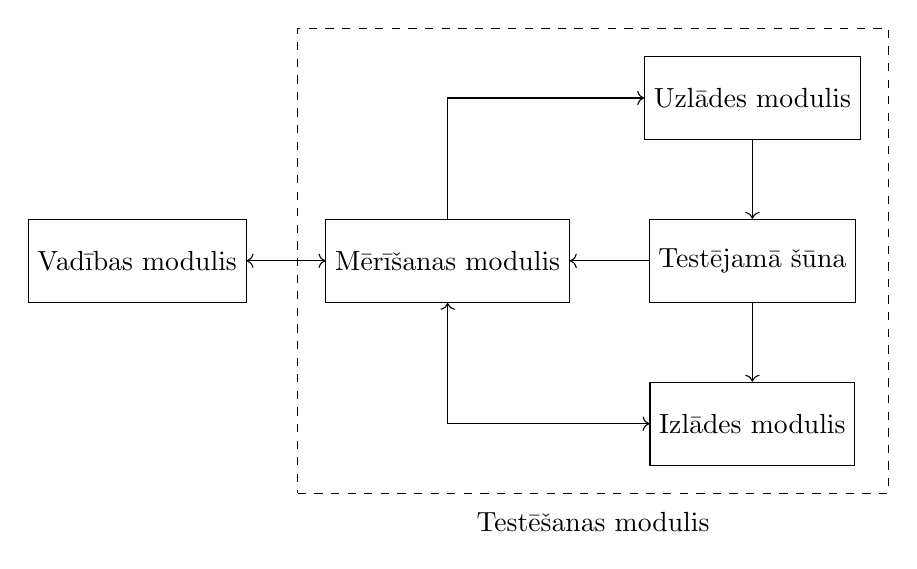
\begin{tikzpicture}
		\node [block] (controller) {Vadības modulis};
		
		\node [block, right=of controller] (mea1) {Mērīšanas modulis};
		\node [block, right=of mea1] (bat1) {Testējamā šūna};
		\node [block, below=of bat1] (disc1) {Izlādes modulis};
		\node [block, above=of bat1] (charge1) {Uzlādes modulis};
				
		\draw [<->] (controller.east) -- (mea1.west);
		\draw [<-] (mea1.east) -- (bat1.west);
		\draw [->] (mea1.north) |- (charge1.west);
		\draw [<->] (mea1.south) |- (disc1.west);
		\draw [->] (bat1.south) -- (disc1.north);
		\draw [<-] (bat1.north) -- (charge1.south);
		
		\node [
			draw=black, 
			dashed, 
			inner sep=1em, 
			fit= (mea1) (bat1) (disc1) (charge1)] (cont1) {};
		\node [yshift=-1em] at (cont1.south) {Testēšanas modulis};
	\end{tikzpicture}
	\caption{Kopējas sistēmas blokshēma}
\end{figure}

\subsection{Mērīšanas modulis}

Sprieguma diapazons $0.00-4.50\pm0.01 V$, strāvas diapazons $0.00-10.00\pm0.05 A$. Temperatūras sensors ar diapazonu $0.0-100.0\degree $. 
Datu nolasīšana izmantojot I2C interfeisu.
Barošanas spriegums $+12VDC$ un $+5VDC$. 
Ar relejiem spēj atslēgs izlādes un uzlādes moduļus no šūnas.

\subsection{Izlādes modulis}

Sākuma spriegums līdz $4.35V$, iestādāms beigu spriegums $2.50-4.35 V$.
Maksimālā izlādes strāva $20(10) A$, jauda $80(40) W$.
Sprieguma, strāvas un temperatūras vērtības tiks nolasītas no mērīšanas moduļa. 

\subsection{Uzlādes modulis}

Ieteicams izmantot IC. Vienas šūnas uzlādes IC ir paradzēti uzlādei no USB, tāpēc ieejas spriegums ir $+5VDC$. USB PD standartiem atbilstoši lādētājiem ir arī ieejas līdz $+22VDC$, bet tam nepieciešama papildu konfigurācija izmantojot USB D+/D-, I2C vai rezistorus.

Parametri:
\begin{itemize}
	\item Iestādāma maksimālā uzlādes strāva līdz 3.5 $A$ (?) %TODO 3.5Ah @ 1C max?
	\item Iestādāms maksimālais spriegums līdz $4.35 V$
\end{itemize}

\subsection{Vadības modulis}

Vad

\FloatBarrier
\newpage
\section{\texorpdfstring{\MakeUppercase{Sistēmas izstrāde}}{Sistēmas izstrāde}}

\subsection{Izlādes modulis}

\subsection{Uzlādes modulis}

\subsection{Vadības modulis}

\subsection{Kopējā sistēma}

\FloatBarrier
\newpage
\section{\texorpdfstring{\MakeUppercase{Secinājumi}}{Secinājumi}}

\FloatBarrier
\newpage

%TODO Fix hyperlink
\addcontentsline{toc}{section}{\texorpdfstring{\MakeUppercase{Izmantotā literatūra}}{Izmantotā literatūra}}
\section*{\texorpdfstring{\MakeUppercase{Izmantotā literatūra}}{Izmantotā literatūra}}
\printbibliography[heading=none]

\FloatBarrier
\newpage
\vspace*{\fill}

%TODO Fix hyperlink
\addcontentsline{toc}{section}{\texorpdfstring{\MakeUppercase{Pielikumi}}{Pielikumi}}
\section*{\centering\texorpdfstring{\MakeUppercase{Pielikumi}}{Pielikumi}}

\vspace*{\fill}
\FloatBarrier
\newpage

\subsection*{1. Pielikums}

\end{document}
